\documentclass[conference]{IEEEtran}
\IEEEoverridecommandlockouts
\usepackage{cite}
\usepackage{amsmath,amssymb,amsfonts}
\usepackage{algorithmic}
\usepackage{flafter}
\usepackage{graphicx}
\usepackage{textcomp}
\usepackage{xcolor}
\graphicspath{ {imagenes/} }

\begin{document}

\title{Actividad G.1\\Pila de Datos
}

\author{\IEEEauthorblockN{Ricardo David López Arellano}
\IEEEauthorblockA{\textit{Departamento de Ingeniería en Computación} \\
\textit{CUCEI}\\
Universidad de Guadalajara\\
ricardo.lopez1361@alumnos.udg.mx}
}
\onecolumn
\maketitle

\begin{abstract}
Una pila es una lista ordinal o estructura de datos en la que el modo de acceso a sus elementos es de tipo LIFO que permite almacenar y recuperar datos. Se aplica en multitud de ocasiones en informática debido a su simplicidad y ordenación implícita en la propia estructura. Representación gráfica de una pila.
\end{abstract}

\begin{IEEEkeywords}
\begin{center}
Drop, Dup, Emit , Print, S, Swap
\end{center}
\end{IEEEkeywords}

\section{Originalidad}

Me comprometo a producir trabajo académico íntegro, lo que significa un trabajo que se adhiere a los estándares intelectuales y académicos de atribución exacta de las fuentes, uso y recolección de datos apropiados, y transparencia en el reconocimiento de las contribuciones de las ideas, descubrimientos, interpretaciones y conclusiones de otros.
Acepto que la trampa en los exámenes, el plagio o la fraudulenta representación de las ideas o lenguaje de otros como propio, la falsificación de datos o cualquier otra instancia de deshonestidad académica, violan los estándares de LA MATERIA, así como los estándares del mundo en general en el campo del conocimiento y las relaciones.

\section{Introducción}
\begin{center}
La pila de datos DS (del inglés, Data Stack), permite efectuar y evaluar operaciones utilizando números enteros (con signo y sin signo), así como símbolos (caracteres).
\end{center}

\section{Objetivos de la actividad}
\begin{center}
 Realizar operaciones aritméticas utilizando la pila de datos.
\end{center}

\section{Metodología}
Una pila (stack en inglés) es una lista ordenada o estructura de datos que permite almacenar y recuperar datos, siendo el modo de acceso a sus elementos de tipo LIFO (último en entrar, primero en salir). Esta estructura se aplica en multitud de supuestos en el área de la informática debido a su simplicidad y capacidad de dar respuesta a numerosos procesos.\\

Para el manejo de los datos cuenta con dos operaciones básicas: apilar (push), que coloca un objeto en la pila, y su operación inversa, retirar (o desapilar, pop), que retira el último elemento apilado.\\

En cada momento solamente se tiene acceso a la parte superior de la pila, es decir, al último objeto apilado. La operación retirar permite la obtención de este elemento, que es retirado de la pila permitiendo el acceso al anterior (apilado con anterioridad), que pasa a ser el último, el nuevo TOS.

\section{Contenido}
\subsection{Operadores de la celda superior:}
\begin{itemize}
\item Drop: palabra que borra la celda superior en la pila de datos.
\item Dup: palabra que duplica el contenido de la celda superior en la pila de datos..
\item Emit: palabra que imprime en la terminal el símbolo que se encuentre en la celda top..
\item Print: palabra que imprime en la terminal el número entero que se encuentra en la celda top..
\item S. : palabra que imprime el número entero con signo que se encuentra en la celda top..
\item Swap: palabra que intercambia las 2 celdas superiores de la pila de datos.
\end{itemize}
\subsection{Operadores de la segunda celda:}
\begin{itemize}
\item Nip: palabra que borra la segunda celda en la pila de datos..
\item Over: palabra que duplica la segunda celda en la pila de datos.
\end{itemize}
\subsection{Operadores de la tercera celda:}
\begin{itemize}
\item Rot: palabra que transfiere la tercera celda a la celda superior en la pila de datos.
\end{itemize}
\subsection{Operadores de la pila de datos:}
\begin{itemize}
\item Depth: palabra que regresa el número de celdas que hay en la pila de datos..
\item DS. : palabra que imprime el contenido de la pila de datos..
\item Pick: palabra que copia la énesima celda en la parte superior de la pila de datos..
\item Roll: palabra que mueve la énesima celda a la parte superior de la pila de datos..
\end{itemize}

\section{Resultados}
\begin{enumerate}
\item  EJERCICIO 1:\\
	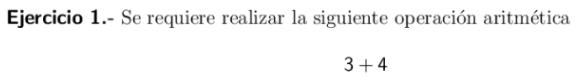
\includegraphics{e1}\\
	\begin{center}
	\textbf{Respuesta: }3 4 + .
	\end{center}
	
\item EJERCICIO 2: \\
	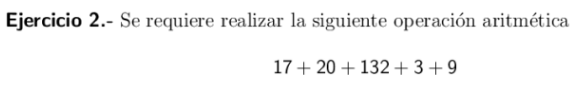
\includegraphics{e2}\\
	\begin{center}
	\textbf{Respuesta: } 17 20 132 3 9 + + + + . 
	\end{center}
	
\item EJERCICIO 3: \\
	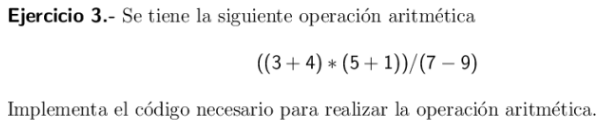
\includegraphics{e3}\\
	\begin{center}
	\textbf{Respuesta: } 3 4 + \\ 5 1 + \\ * \\ 7 9 S- //Colocar esa letra sirve imprimir numeros negativos \\ S/ \\ S.
	\end{center}	
	
\item EJERCICIO 4.1: \\
	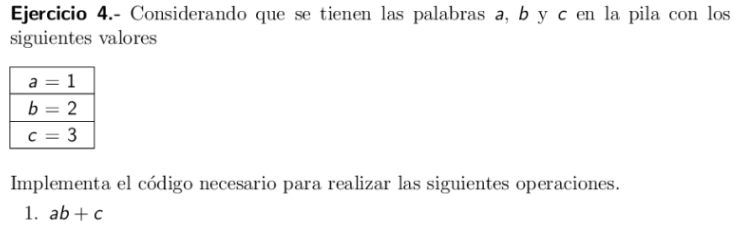
\includegraphics{e4.1}
	\begin{center}
	\textbf{Respuesta: } c 3 b 2 a 1 \\ a b + \\ c + \\ .
	\end{center}	
	
\item EJERCICIO 4.2: \\
	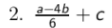
\includegraphics{e4.2}
	\begin{center}
	\textbf{Respuesta: } c 3 b 2 a 1 \\ swap 4 * //intercambiar las 2 celdas superiores para poder hacer la multiplicación \\ S- \\ 6 S/ \\ S+ \\ .
	\end{center}	
	
\item EJERCICIO 4.3: \\
	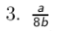
\includegraphics{e4.3}
	\begin{center}
	\textbf{Respuesta: } c 3 b 2 a 1 \\ swap 8 * //intercambiar celdas \\ / \\ nip //borrar la segunda celda \\ .
	\end{center}	
	
\item EJERCICIO 4.4: \\
	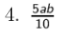
\includegraphics{e4.4}
	\begin{center}
	\textbf{Respuesta: } c 3 b 2 a 1 \\ a b * \\ 5 * \\ 10 / \\ .
	\end{center}
	
\item EJERCICIO 4.5: \\
	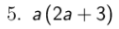
\includegraphics{e4.5}
	\begin{center}
	\textbf{Respuesta: } c 3 b 2 a 1 \\ tuck \\ 2 * \\ 3 + \\ swap //intercambiamos las celdas \\ drop //borramos la celda superior \\ * \\ .
	\end{center}
	
\item EJERCICIO 4.6: \\
	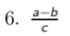
\includegraphics{e4.6}
	\begin{center}
	\textbf{Respuesta: } c 3 b 2 a 1 \\ swap //intercambiamos las celdas \\ b / \\ +S \\ . \\ 
	\end{center}	
	
\end{enumerate}

\section{Conclusiones}  
En conclusión de esta tarea puedo decir que estos ejercicio fueron demasiados fáciles ya que no tenia mucha lógica realizarlos, pero como hemos ido avanzando se fueron complicando más. Pero es bueno aprender un lenguaje nuevo ya que yo ni si quiera había utilizado Linux ni mucho menos Latex, así que es una buena experiencia.

\section*{Agradecimientos}
Quiero hacer agradecimiento a mi profesor por explicarme cuando tenia dudas sobre cómo hacer los ejercicios, a mis compañeros porque varias veces me brindaron ayuda cuando tenia problemas y a mis padres en apoyarme cuando los necesito.

\begin{thebibliography}{00}
\bibitem{Alvarez2022} Becerra Alvarez, E. C. (2022, 4 octubre). ForEmb. Classroom.google.com. https://drive.google.com/file/d/126erNsd5G0STuELmVFfrtDviOSrzSwGC/view
\end{thebibliography}

\end{document}
